\documentclass{article}

% if you need to pass options to natbib, use, e.g.:
% \PassOptionsToPackage{numbers, compress}{natbib}
% before loading nips_2016
%
% to avoid loading the natbib package, add option nonatbib:
% \usepackage[nonatbib]{nips_2016}

\usepackage[final]{nips_2016}

% to compile a camera-ready version, add the [final] option, e.g.:
% \usepackage[final]{nips_2016}

\usepackage[utf8]{inputenc} % allow utf-8 input
\usepackage[T1]{fontenc}    % use 8-bit T1 fonts
\usepackage{hyperref}       % hyperlinks
\usepackage{url}            % simple URL typesetting
\usepackage{booktabs}       % professional-quality tables
\usepackage{amsfonts}       % blackboard math symbols
\usepackage{nicefrac}       % compact symbols for 1/2, etc.
\usepackage{microtype}      % microtypography
\usepackage{subfigure}
\usepackage{svg}
\usepackage[ruled,vlined]{algorithm2e}

\usepackage{graphicx}

% Macros
\newcommand{\R}{\mathbb{R}}



\title{Graphs for Machine Learning Project (MVA)\\Convolutional Neural Network on Graphs}

% The \author macro works with any number of authors. There are two
% commands used to separate the names and addresses of multiple
% authors: \And and \AND.
%
% Using \And between authors leaves it to LaTeX to determine where to
% break the lines. Using \AND forces a line break at that point. So,
% if LaTeX puts 3 of 4 authors names on the first line, and the last
% on the second line, try using \AND instead of \And before the third
% author name.


\author{Alexandre~P\'er\'e \And Cl\'ement~Tiennot}

\begin{document}
% \nipsfinalcopy is no longer used

\maketitle

\begin{abstract}
    In this report, we present our understanding of the paper "Convolutional Neural Networks on Graphs with Fast Localized Spectral Filtering" \cite{defferrard2016convolutional}. We both summarize the approach developed in the authors' work and provide an implementation in the \texttt{python} langage. Our implementation makes use of the \texttt{Tensorflow} package \cite{tensorflow2015-whitepaper} which allows automatic computation of gradients and thus efficient optimization.
\end{abstract}



%\section*{Pseudo-Algorithms}

We need to implement the following methods:
\begin{itemize}
    \item Convolution of a signal on a graph with parameter $\theta$
    \item Graph coarsening of a graph
    \item Computation of gradient w.r.t. filter parameters
    \item Backpropagation of gradient through coarsening operation
\end{itemize}


\begin{algorithm}[ht]
 \KwData{input signal $x \in \R^d$, filter parameters $\theta \in \R^K$ , Graph Laplacian $L_\mathcal{G} \in \R^{d \times d}$}
 \KwResult{filtered signal $y \in \R^d $}
 
 \textbf{Initialization:}\\
    $\tilde{L} = 2 L / \lambda_{max} - I_d$ \\
    $\bar{x}_0 = x$ \\
    $\bar{x}_1 = \tilde{L}x$
 
 \For{$k=2$ to $K-1$}{
    $\bar{x}_k=2\tilde{L}\bar{x}_{k-1} - \bar{x}_{k-2}$
 }
 \textbf{Return:} $y = [\bar{x}_0, \ldots, \bar{x}_{K-1}] \theta$
 \caption{Fast localized spectral filter}
\end{algorithm}  % some stuff that we will need to put somewhere later

\section*{Introduction}

Lately, Convolutional Neural Networks (CNN), have shown outstanding performances in classification tasks over a large range of data including images, audio and language. Those techniques are rapidly spreading across the scientific community, leading to unprecedented advances in different fields. Even though those performances are quite promising for future applications, the generalization of CNN to discrete signals over arbitrary (non-euclidean) structure is still an open problem. Indeed, it is worth noting that the data on which CNN give their best performances share an important common property: they all can be represented as contiguous data over regular lattices, like regular 2D arrays for images, or regular 1D arrays for sequences. 

The convolution operation that confers their performances to CNN can be seen from two different viewpoints:
\begin{itemize}
    \item The convolution operation is equivalent to a multiplication in the Fourier domain. This definition is not the most intuitive and is, to our knowledge, rarely used in practical implementations due to the cost of transferring data to the complex Fourier domain. 
    \item The convolution operation is also equivalent to a classic filtering with a small sliding window, scanning and filtering the whole input signal (in the case of images, the filter can be a small 3x3 filter called kernel). This definition is much meaningful to understand the way CNN behaves, and is most often used for implementation.
\end{itemize}

From these two definitions, we understand that CNN performance relies heavily on the euclidean structure of the data, and the idea of locality and neighbourhood. Thus, it becomes clear that CNN can't be easily applied to data presenting less structure than images or sequences, for example in the case of signals defined over sensor fields, or trees.

The main question addressed by the paper is hence: How do we apply CNN to more general discrete signals over non-euclidean structures where straightforward convolution operation can not be defined. Graphs structure being the most general discrete structure we can define signals on, this question extends to: How do we apply CNN to signals defined over graphical structures? 

In order to address this issue, we will have to rely on the Fourier Domain multiplication point of view. As we will see, one can use a spectral approach to define Fourier Transform over graphs, along with convolutions and filtering \cite{bruna2013spectral}. By choosing a specific filter parametrization (that uses the graph Laplacian) we can furthermore build localized and fast filters with performances comparable to classic CNN.

The Graph CNN implementation proposed in the paper is made possible by theoretic tools provided by the emerging field of Graph Signal Processing (GSP). This new field aims at studying discrete signals over non-euclidean structures, and is rapidly gaining attraction in the signal processing community. A complete introduction to the field can be found in \cite{Shuman2013}.




\section{A bit of Graph Theory}

A weighted graph is defined as a tuple $(\mathcal{V,E,W})$, where $\mathcal{V}$ is a set of elements called Vertices (or Nodes), $\mathcal{E}$ is a set of couples of $\mathcal{V}$ elements called Edges (or Arcs), and $\mathcal{W: E}\rightarrow \mathbb{R}$ is an application that assigns weights $w$ to all edges. 

Most of the time, the application $\mathcal{W}$ is represented by a \emph{Weight matrix} $W$, which, if we consider a $n$ nodes graph, is an $n\times n$ matrix. If an edge exists between two nodes $i,j \in \mathcal{V}$, then $w_{ij}\neq 0$, and if no edge exists then $w_{ij}=0$. A graph can be directed or undirected. In our case we will exclusively use undirected graphs, meaning that the weights matrix is always symmetric. The \emph{Degree} of a node $i$ is defined as the sum of the weights related to it:
\begin{equation}
    d_i = \sum_{k\in\mathcal{V}}w_{ik}    
\end{equation}
The \emph{Degree matrix} $D$ of a graph is a $n\times n$ diagonal matrix containing the degrees of all nodes $i$.

With these definitions we can introduce one of the most interesting tools used in graphs for machine learning, the graph \emph{Laplacian matrix}, which is defined as:
\begin{equation}
    L = D -W
\end{equation}
This matrix is a fruitful representation of a graph that has a lot of interesting properties. In the case of Graph Fourier Transform that we will define in the next part, a slightly different definition of the Laplacian is used, i.e. the symmetric normalized Laplacian:
\begin{equation}
    L_{sym} = D^{-1/2}LD^{-1/2}
\end{equation}
Other definitions of the Laplacian can be found in the literature, having each different and interesting properties that we will not discuss here. For more insights on graph Laplacian and spectral clustering, one can refer to \cite{VonLuxburg2007}.

Last but not least, a discrete signal $s$ over a graph $\mathcal{G}$ is defined as an application $s:\mathcal{V}\rightarrow \mathbb{R}$, that maps a real number to each graph nodes. In what follows, we will refer to such discrete signals over graphs, merely as signals.
 

\section{Spectral filter on graph}

In this section we introduce spectral filtering of signals defined over a graph. 

\subsection{Spectral domain}

For a graph $G = (V, E, W)$ with Laplacian $L \in \R^{n\times n}$, we have the following spectral decomposition, with $U \in \R^{n\times n}$ the change of basis matrix that diagonalizes the Laplacian $L$:
%
\begin{equation}
    L = U \Lambda U^T \quad \mathrm{with} \quad \Lambda = \mathrm{diag}([\lambda_0, \dots, \lambda_{n-1}])
\end{equation}
%
The authors then introduce the Graph Fourier Transform (GFT) which takes a spatial one-dimensional signal (defined on the nodes of G) $x \in \R^n$ and maps it to its counterpart in the spectral domain $\hat x = U^T x \in \R^n$. The inverse operation $x = U \hat x$, allows to switch between the spatial on spectral domain at ease, provided the Fourier basis $U$ is known.

On figure \ref{fig:fourier_modes} we can see plots of some of the Laplacian eigenvectors over a regular 2D grid graph. We can see that those Fourier modes define complex periodic patterns, that shows quite clearly why the Laplacian eigendecomposition can be used as a Graph Fourier Transform.

\begin{figure}
    \centering
    \subfigure[mode 91]{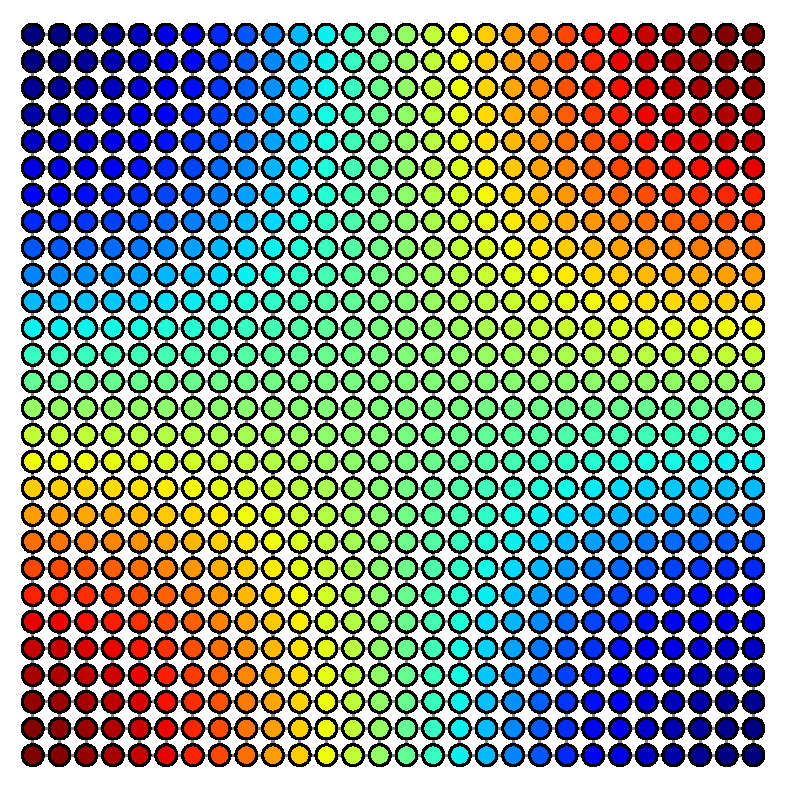
\includegraphics[width=0.24\textwidth]{img/mode3.pdf}}
    \subfigure[mode 215]{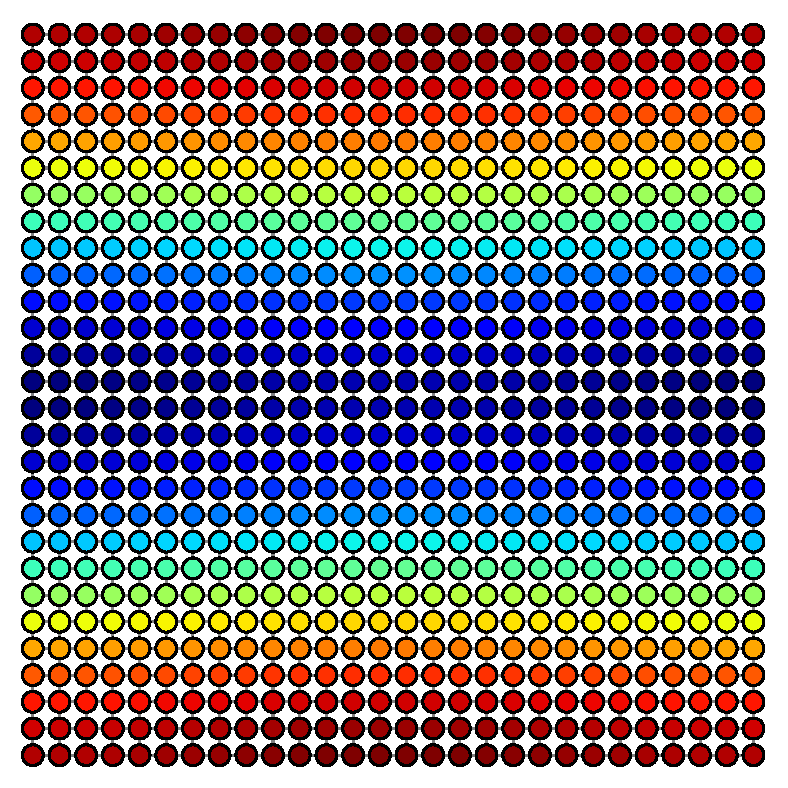
\includegraphics[width=0.24\textwidth]{img/mode5.pdf}}
    \subfigure[mode 474]{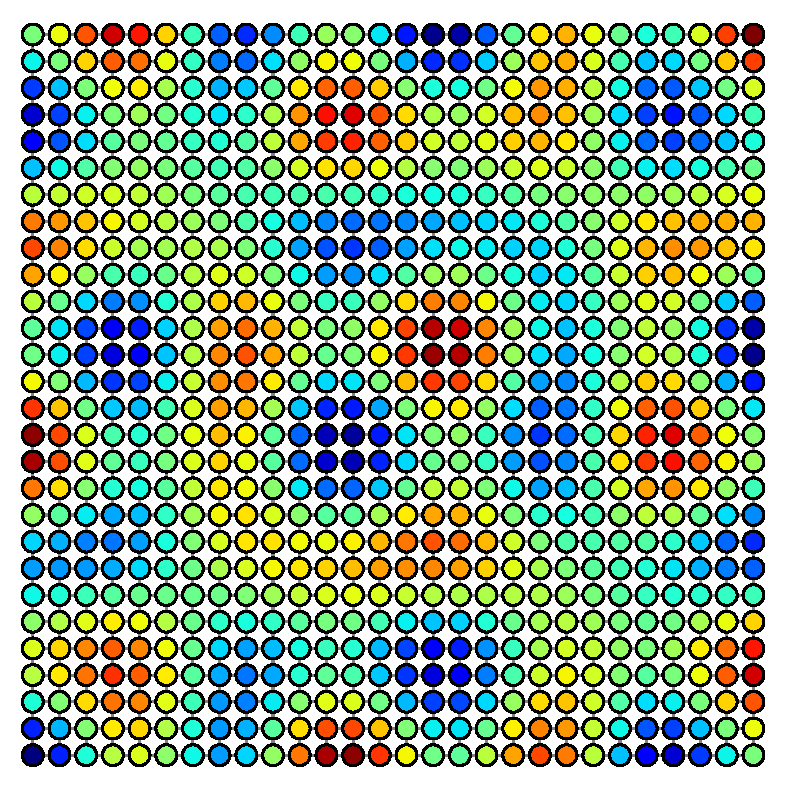
\includegraphics[width=0.24\textwidth]{img/mode50.pdf}}
    \subfigure[mode 613]{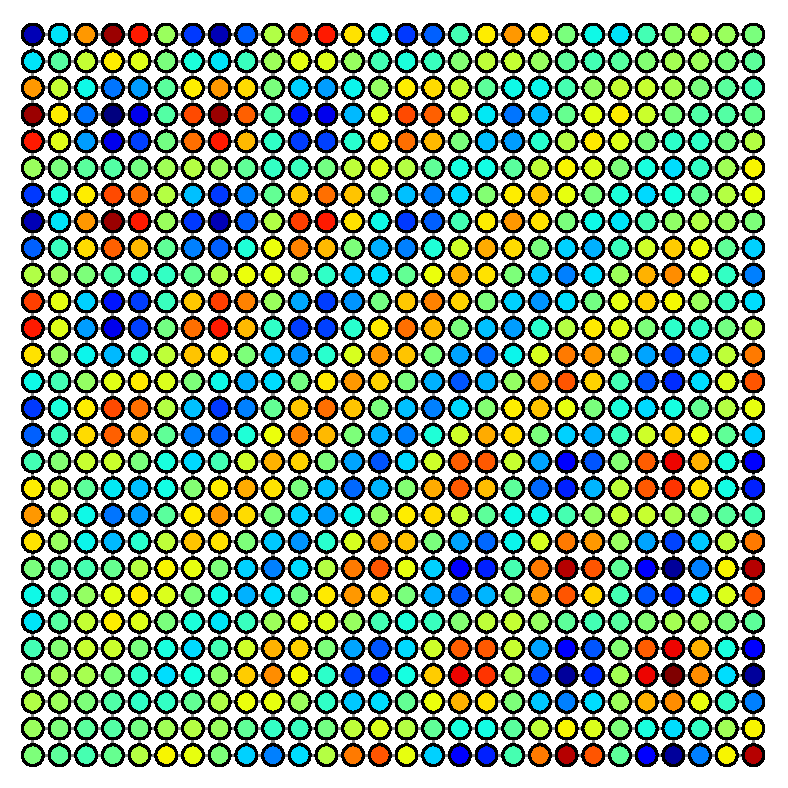
\includegraphics[width=0.24\textwidth]{img/mode100.pdf}}
    \caption{Some Fourier Modes plotted over the graph (i.e. Laplacian eigenvectors)}
    \label{fig:fourier_modes}
\end{figure}


\subsection{Filtering}

Applying a filter in the spatial domain amounts to perform an element-wise product in the spectral domain. Hence we can take a filter operator $g_\theta(.)$ that is defined in the spectral domain (and depends on some parameter vector $\theta$) and apply it to $\bar x$: the output in the spectral domain is then $\bar y = g_\theta \bar x = g_\theta U^T x$. To get the final filtered signal $y$ we go back to the spatial domain using the inverse GFT:
%
\begin{equation}
    y = U \bar y = U g_\theta  U^T x
\end{equation}
%
In practice the element wise product of $U^T x$ by all the components of the filter $g_\theta$ can be achieved as a matrix multiplication if we define our filter as a diagonal matrix in $\R^{n\times n}$. It follows that any filter is of the form $\mathrm{diag}(\theta)$ with $\theta \in \R^n$. The authors refer to this general construction as a \textit{non-parametric filter} because it has the maximum allowed degrees of freedom.

\subsection{Localized filters}

As pointed out by the authors, this general formulation is not satisfactory because it is not localized in space (each component of the output signal depends on every component of the input signal) and the number of parameters to learn is equal to the signal size which is a bottleneck and is not the case for standard convolutional filters on images.\\

One can show \cite{hammond2011wavelets} that if the shortest path between two vertices $i$ and $j$ on the graph is strictly greater than $K$ then $(L^K)_{i,j} = 0$. A natural idea that then arises is to design a filter that is parametrized over powers of the Laplacian (or in the spectral domain, the powers of $\Lambda$) to control the spatial localization of the filter:
%
\begin{equation}
    g_\theta(\Lambda) = \sum_{k=0}^{K-1} \theta_k \Lambda^k \label{eq:localized_filter}
\end{equation}
%
Thus using the previously stated property it is easy to prove the spatial $K-$localization of such filters (see the original paper). In addition the learning complexity is now independent of the signal size since we only have $K$ parameters. 

Figure \ref{fig:filtered} shows an MNIST "9" sample filtered using different powers of the Laplacian. We can see that depending on K, only some large areas of stationary signals are kept, while the rest is discarded from the representation.

\begin{figure}
    \centering
    \subfigure[$\Lambda^1$]{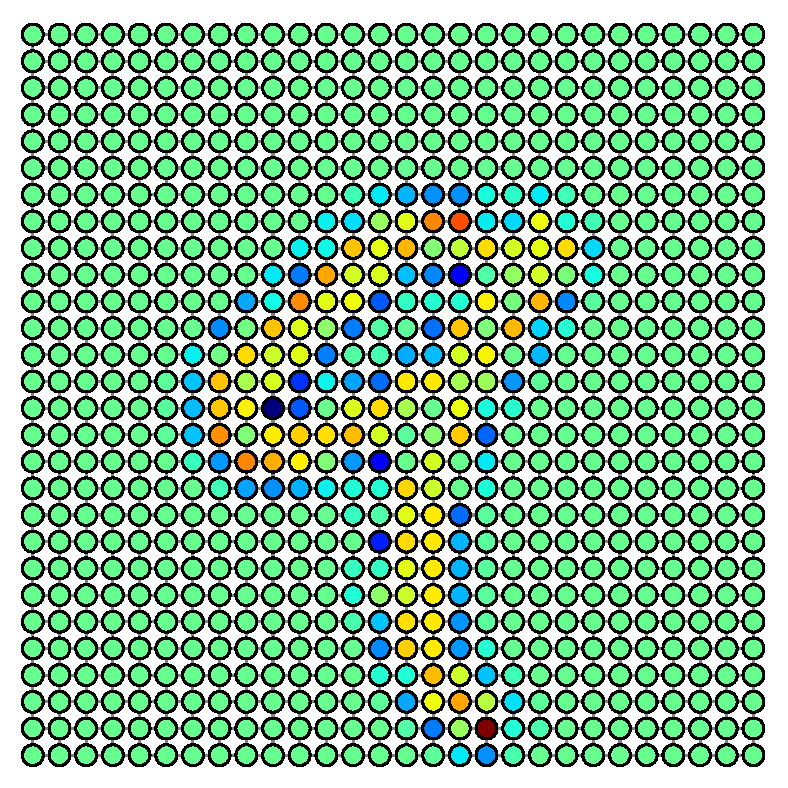
\includegraphics[width=0.24\textwidth]{img/L1.pdf}}
    \subfigure[$\Lambda^3$]{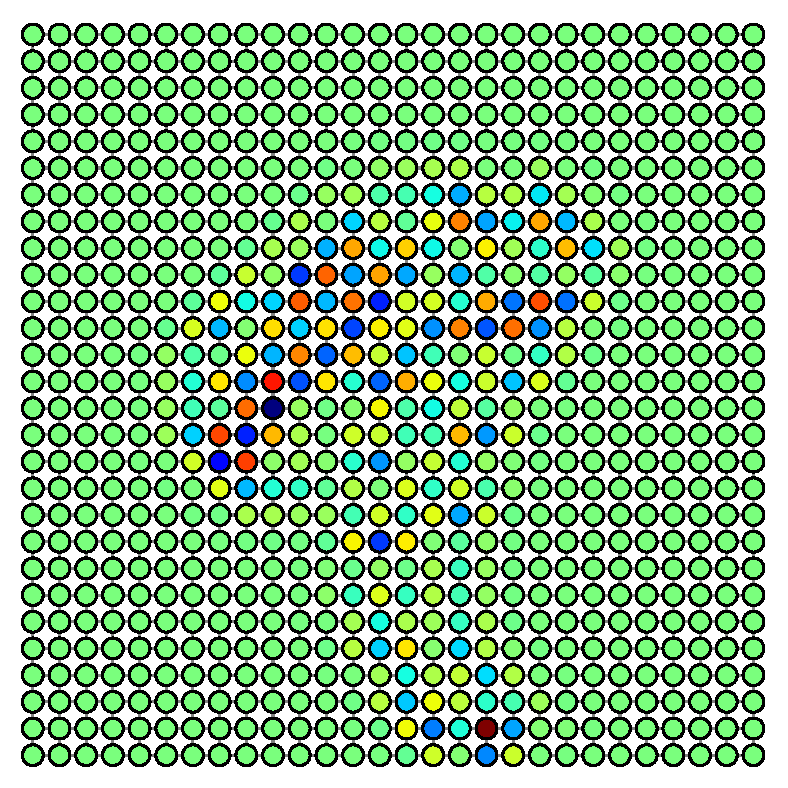
\includegraphics[width=0.24\textwidth]{img/L3.pdf}}
    \subfigure[$\Lambda^5$]{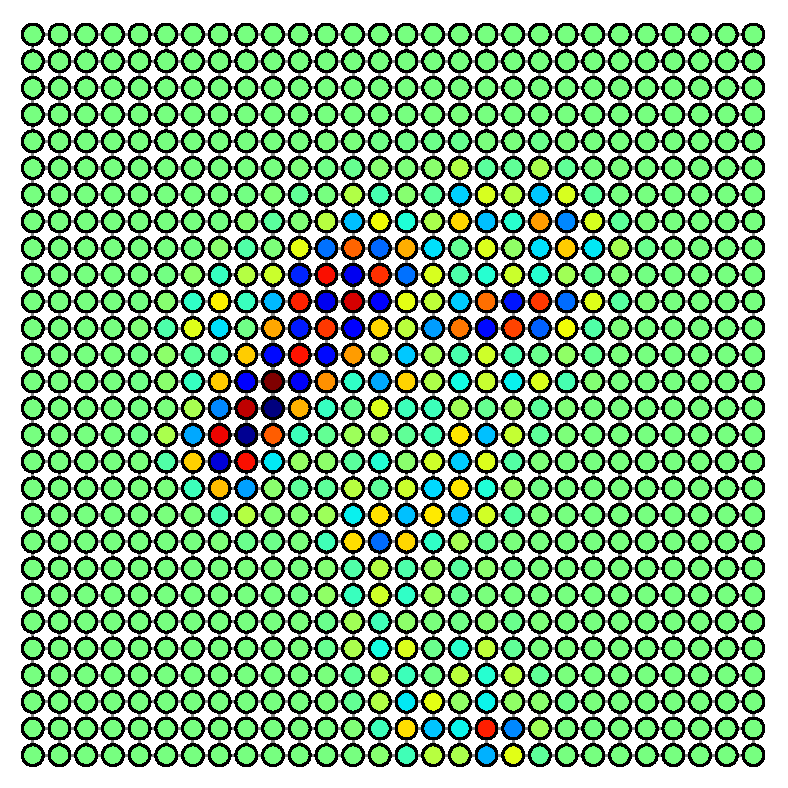
\includegraphics[width=0.24\textwidth]{img/L5.pdf}}
    \subfigure[$\Lambda^9$]{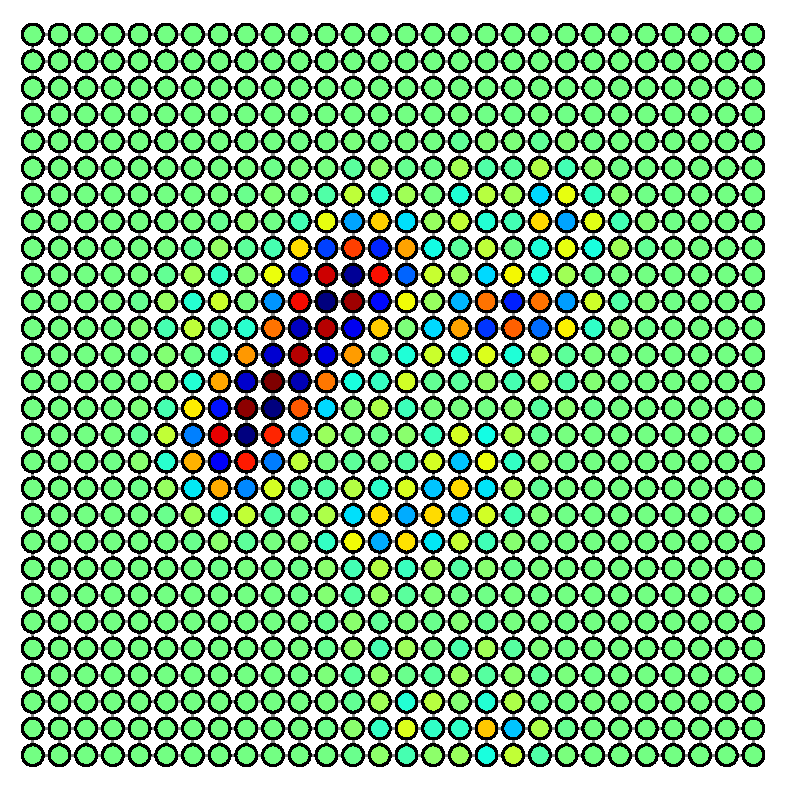
\includegraphics[width=0.24\textwidth]{img/L8.pdf}}
    \caption{Localized filtering of a signal using different powers of $\Lambda$.}
    \label{fig:filtered}
\end{figure}

\subsection{Fast filtering or Chebyshev approximated filters}
%
Equation \ref{eq:localized_filter} is the theoretical key to construct a CNN on a graph, but for an efficient implementation it has one downside: in practice switching between the spatial and the spectral domain implies two matrix multiplications by $U^T$ and $U$ (which are dense matrices) and has a cost $\mathcal{O}(n^2)$. The authors, thus, make use of the Chebyshev polynomial approximation $T_k(x)$ defined recursively by $T_k(x) = 2xT_{k-1}(x) - T_{k-2}(x)$ with $T_0=1$ and $T_1 = x$ which forms an orthogonal basis of $L^2([-1,1])$ with respect to the weights $1/\sqrt{1 - x^2}$. The proposed filter is then defined as:
\begin{equation}
    g_\theta(\Lambda) = \sum_{k=0}^{K-1} \theta_k T_k(\tilde \Lambda) \label{eq:localized_filter}
\end{equation}
%
Where $\tilde \Lambda = 2\Lambda / \lambda_max - I_n$ is the scaled diagonalized Laplacian whose coefficients lie in $[-1, 1]$. Because each $T_k$ has degree $k$, this is a re-parametrization of equation \ref{eq:localized_filter} which proves directly the spatial localization. Finally the authors explicit the output signal y as $y = g_\theta(L)x = \sum_{k=0}^{K-1} \bar x_k$ with $\bar x_k = \theta_k T_k(\tilde L) x$. The $\bar x_k$'s can be computed by the recursion $\bar x_k = 2 \tilde L \bar x_{k-1} - \bar x_{k-2}$ with $\bar x_0 = x$ and $\bar x_1 = \tilde L x$. The filtered signal is then given by $y = [\bar x_0, \dots, \bar x_{K-1}]\theta$ and the filtering cost is $\mathcal{O}(K|E|)$ because the matrix products during the recursion involve a sparse matrix (the scaled Laplacian) and dense vectors. Algorithm \ref{alg:filtering} summarizes how to perform the filtering. \footnote{Our implementation doesn't benefit from the Laplacian sparsity since our goal was just to demonstrate our understanding of CNN on graphs and not to produce scalable code.}\\

\begin{algorithm}[ht]
 \KwData{input signal $x \in \R^d$, filter parameters $\theta \in \R^K$ , Graph Laplacian $L_\mathcal{G} \in \R^{d \times d}$}
 \KwResult{filtered signal $y \in \R^d $}
 
 \textbf{Initialization:}\\
    $\tilde{L} = 2 L / \lambda_{max} - I_d$ \\
    $\bar{x}_0 = x$ \\
    $\bar{x}_1 = \tilde{L}x$
 
 \For{$k=2$ to $K-1$}{
    $\bar{x}_k=2\tilde{L}\bar{x}_{k-1} - \bar{x}_{k-2}$
 }
 \textbf{Return:} $y = [\bar{x}_0, \ldots, \bar{x}_{K-1}] \theta$
 \caption{Fast localized spectral filter}
 \label{alg:filtering}
\end{algorithm}

\begin{figure}
    \centering
    \subfigure[$T_1$]{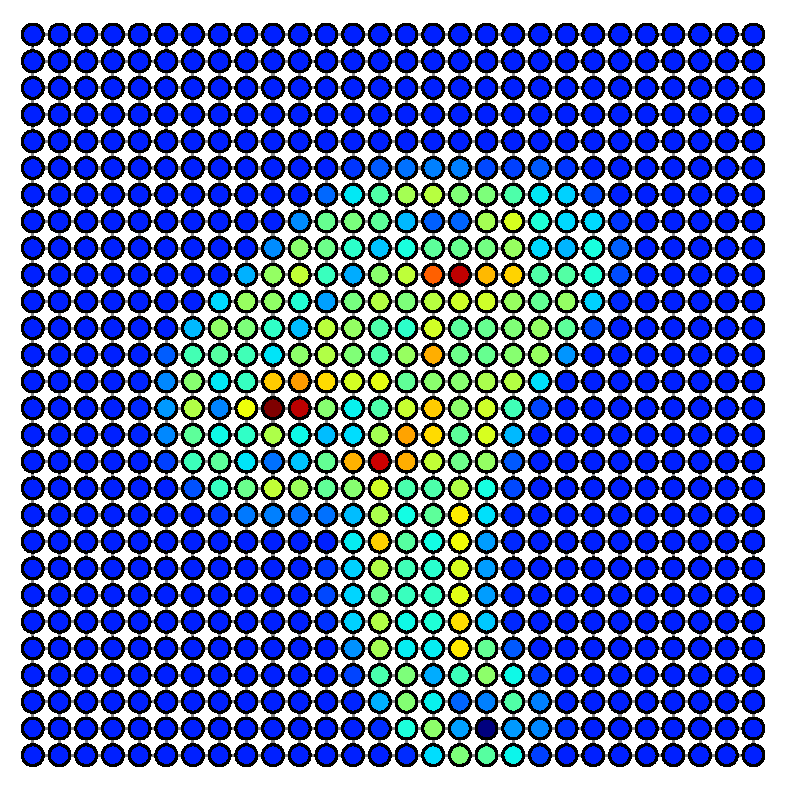
\includegraphics[width=0.24\textwidth]{img/C0.pdf}}
    \subfigure[$T_2$]{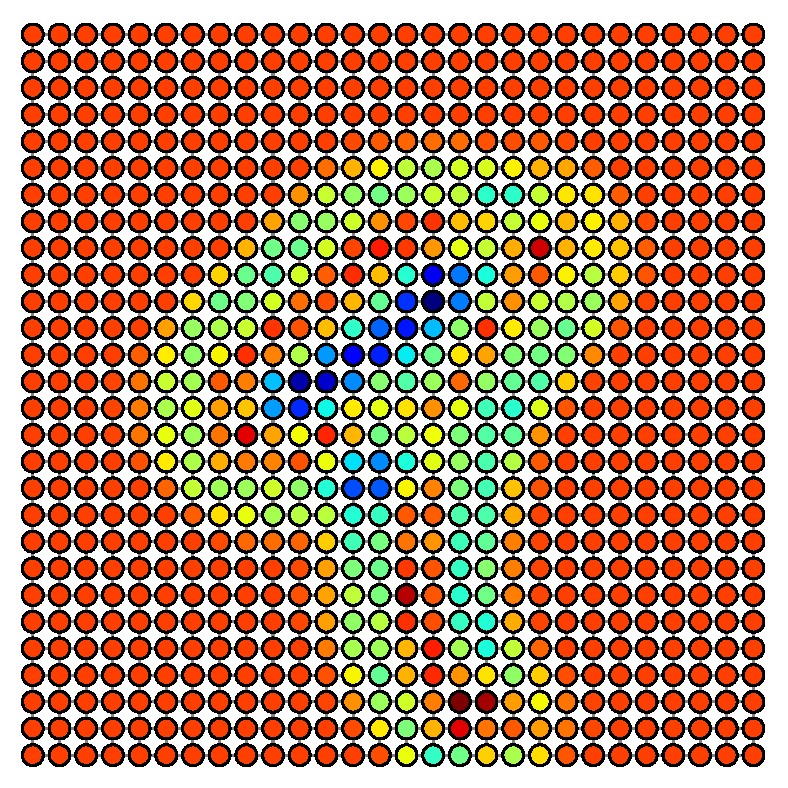
\includegraphics[width=0.24\textwidth]{img/C1.pdf}}
    \subfigure[$T_3$]{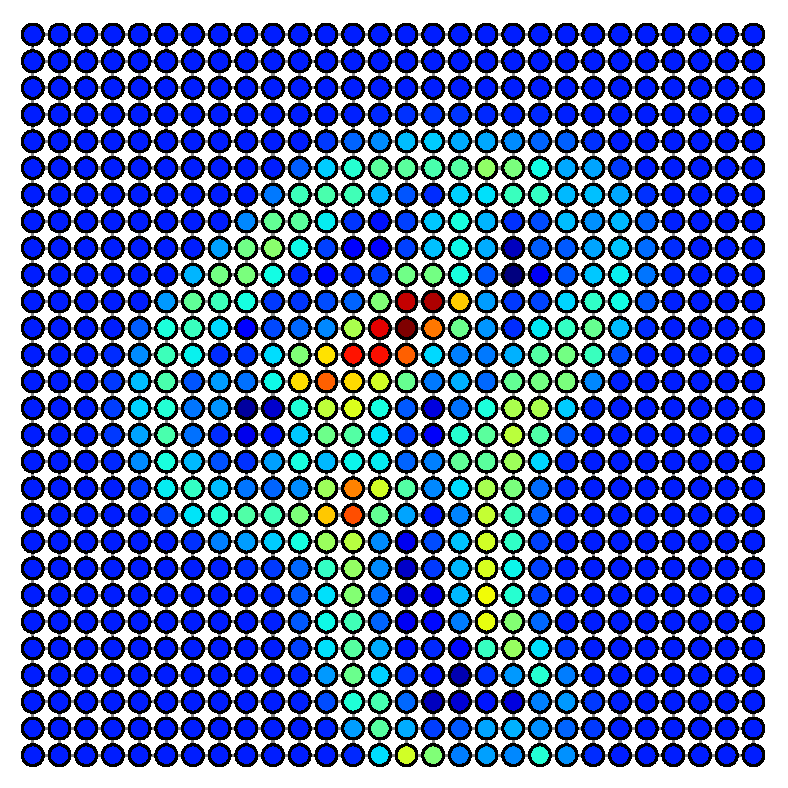
\includegraphics[width=0.24\textwidth]{img/C2.pdf}}
    \subfigure[$T_5$]{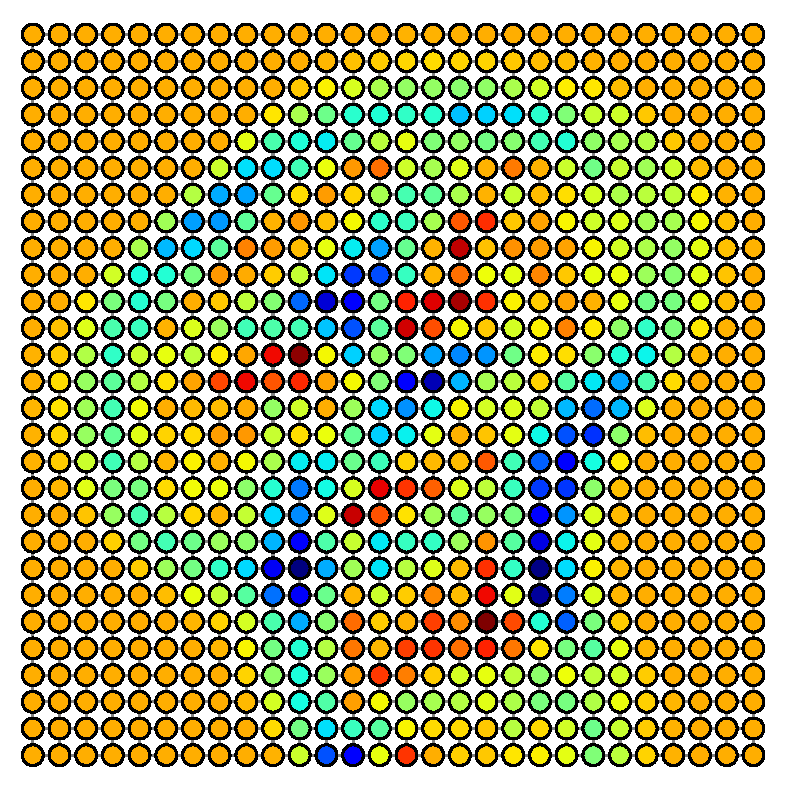
\includegraphics[width=0.24\textwidth]{img/C5.pdf}}
    \caption{Localized filtering of a signal using different orders of Chebyshev approximation.}
    \label{fig:chebyshev_filtered}
\end{figure}

On figure \ref{fig:chebyshev_filtered}, we represented signals filtered using the recursive Chebyshev approximation. The behaviour here is different from the one we had with powers of $\Lambda$, and we can see that the difference formulation of the Chebyshev approximation tends to keep only the boundaries of the signal.

Learning the filters parameters can be achieved using back-propagation and gradient descent (see p.4 of \cite{defferrard2016convolutional} for the gradient expressions). Nevertheless, in our implementation, \texttt{Tensorflow} performs symbolic operations and is able to compute the parameter derivatives automatically which makes it really easy to implement the whole gradient descent even after cascading several filters.\\

An example of filtered signals is given by Figure~\ref{fig:inversed_learnt}: the graph is a grid where each pixel is a node and is connected to its 8 neighbors. On top of this graph the signal is the intensity of each pixel. We randomly chose $K=100$ parameters for a filter and applied it to the signal using the Chebitchev formulation. As expected the filtered signal (left) is blurry. Just to demonstrate the gradient descent using \texttt{Tensorflow}, we tried to retrieve the initial signal (our "9" digit) from the filtered version to see if it is possible to learn an "inverse" filter. After 10~000 iterations of gradient descent, the mean squared error had fallen under 0.04 (i.e. about 20\% average deviation since we normalized the intensity between 0 and 1). The reconstructed signal is far from perfect due to the loss of information during the first filtering but we clearly distinguish the shape of the "9".

\begin{figure}
    \centering
    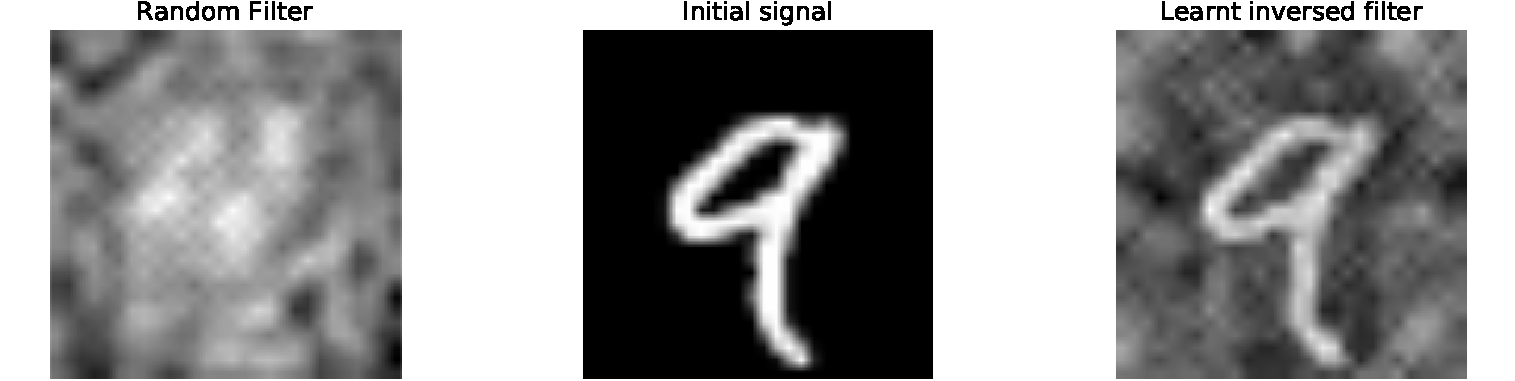
\includegraphics[width=\textwidth]{img/inversed_learnt.pdf}
    \caption{Left: filtered signal with $K=100$ random coefficients. Center: initial signal on the grid graph. Right: filtering of the left signal after having learnt $K=100$ coefficients to create an "inverse" filter using gradient descent.}
    \label{fig:inversed_learnt}
\end{figure}

\section{Efficient Max-Pooling on Graphs}

An important feature of CNNs is their ability to downscale the input information along the network, into a lower dimensional embedding that contains most of the semantic information present in the input. In classic CNNs, this dimension reduction results of two facts:
\begin{itemize}
    \item The Max Pooling Operation: This operation slides a small window (2x2 pixels for images) over the whole input data, and keeps the maximum value in the window.
    \item The Convolution Operation: The convolution operation has the side effect to lower the dimension if the input is not zero padded. 
\end{itemize}

Doing the same on a graph is a bit trickier; for example, the convolution operation used has no effects on the dimension, hence the importance to implement a Graph Max Pooling operation. The authors used a Graph coarsening routine from the Graclus multilevel clustering algorithm \cite{dhillon2007weighted}, to implement this behavior. They then describe an interesting way to re-index the graph nodes (adding extra "virtual" nodes) to allow performing all pooling operations as for a 1 dimensional signal. 

\subsection{Graph coarsening}

The proposed method groups nodes by pairs, dividing the size of the graph by approximately two (some nodes can end up alone). It basically follows the steps:
%
\begin{itemize}
    \item Randomly pick up one non-paired node and look at all its unpaired neighbors to find the one that maximizes a given local cut (the normalized cut $W_{ij}(1/d_i + 1/d_j)$ in our case).
    \item If for a node there are no remaining neighbors to pair it with, then we leave it alone.
    \item Build a new graph where every found pair of nodes becomes a single node
    \item The weights are summed so that if $(i_1, i_2)$ and $(j_1, j_2)$ are two pairs of "old" nodes then the two new nodes ${i}$ and ${j}$ share an edge with weight $W_{ij} = W_{i_1 j_1} + W_{i_1 j_2} + W_{i_2 j_1} + W_{i_2 j_2}$.
\end{itemize}
%
A signal on the initial graph can be max-pooled by taking the maximum value of every pairs of nodes to assign it to the corresponding node in the coarsest graph.\\

Since the coarsening operation approximately reduces the size of the graph by two we can perform it twice to reduce the size by approximately four in a similar way to 2d max-pooling. The nested coarsened versions of the initial graph can be computed once and stored as their Laplacians along with some transition matrices that indicate how to pass from one graph to its coarsest (or backward, finest) version. An illustration of max-pooling using graph coarsening for one MNIST digit is given by Figure~\ref{fig:coarsening}.

\begin{figure}
    \centering
    \subfigure[784 nodes]{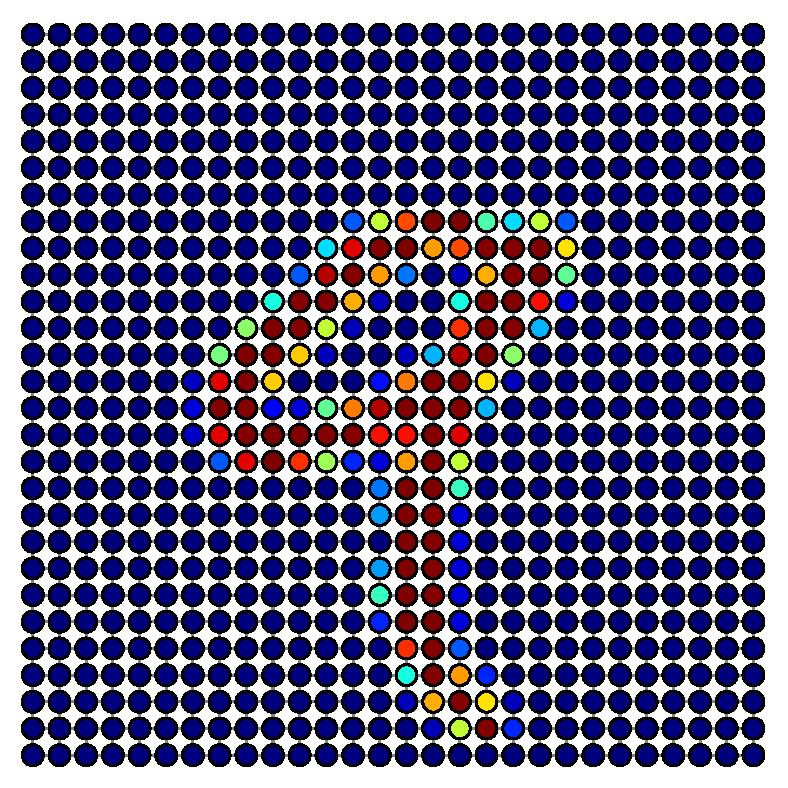
\includegraphics[width=0.24\textwidth]{img/coarsening0.pdf}}
    \subfigure[424 nodes]{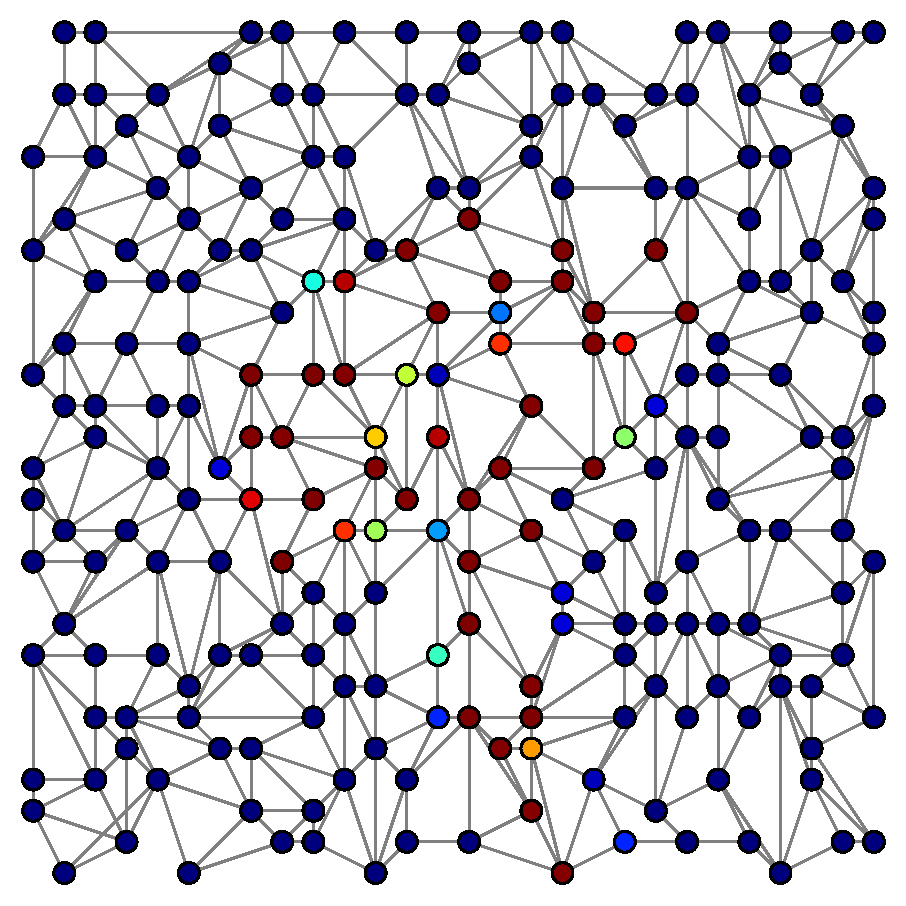
\includegraphics[width=0.24\textwidth]{img/coarsening1.pdf}}
    \subfigure[229 nodes]{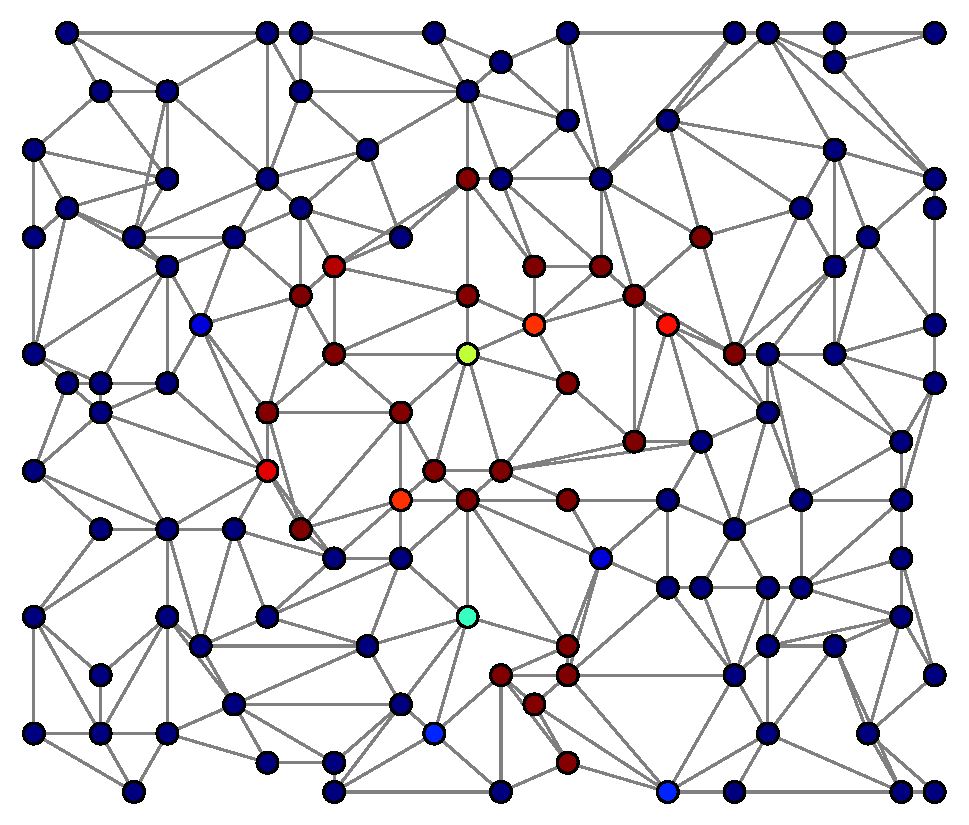
\includegraphics[width=0.24\textwidth]{img/coarsening2.pdf}}
    \subfigure[127 nodes]{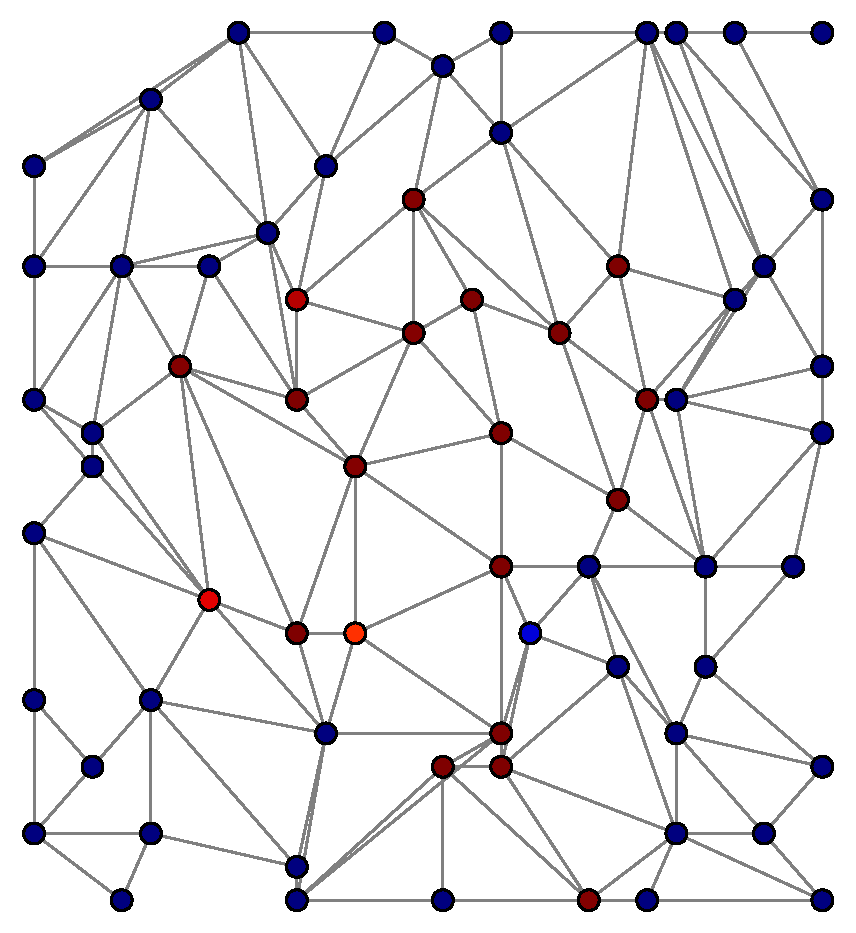
\includegraphics[width=0.24\textwidth]{img/coarsening3.pdf}}
    \caption{Example of pooled signal on four consecutive coarsened versions of an initial grid graph. The initial graph had $28\times28=784$ pixels/nodes. The spatial location of paired nodes was set to be the barycentre of the two initial node positions.}
    \label{fig:coarsening}
\end{figure}

\subsection{Nodes re-indexing to perform fast pooling}

Even though this implementation using transition matrices is effective and allows us to decipher the pooled signals into graph representation, it is not particularly interesting in terms of computational performance (element wise matrix multiplication). To tackle this, we note that once we have obtained all the coarsened version of the initial graph (e.g. 4 or 5 of them), it is possible to reorder the nodes in a smart way that allows us to use a simple 1-D max pooling. We first assign arbitrary numbers to the nodes at the coarsest level. Then each node has either one or two parents and we add "virtual" nodes which will have 0 value (since we use a RELU activation after each convolutional layer they won't change the signal) so that each node has exactly two parents. We then number the nodes at the second coarsest level so that parents are side by side. We then repeat the process until we reach a numbering for nodes in the initial graph (and additional virtual nodes). It should be noted that adding a virtual node at one level implies adding 2 virtual nodes as its parents at the above level and then 4 virtual nodes to be the parents of the two parents and so on. Nevertheless in practice we don't need more than about 6 or 8 coarsened version of the graph so this stays manageable.\\

With the obtained numbering for the nodes of the initial graph, and after having added the virtual nodes, we can perform the pooling operation like a regular 1d pooling because two nodes to be aggregated together will always be side by side. In practice this is really convenient: the ordering just has to be computed once, we then just add the needed fake nodes (with 0 signal values) and rearrange the data. Then all max-pooling operation can be performed as if the signal was one-dimensional.

\section{Putting it altogether: building and training a CNN on graphs}

In order to test our understanding of the algorithms and to gain intuition about the potential of GCNN on classic Neural Network tasks, we have implemented the different algorithms presented in the paper. When coming to Neural Networks, two experiments allow to rapidly gain intuition about the potential of an architecture:
\begin{itemize}
    \item Classification: Check that the architecture proposed is able to classify a simple data-set with acceptable performance.
    \item AutoEncoders : Construct an encoder-decoder architecture to verify that the model allows to construct interesting embedded representation of simple data. 
\end{itemize}

Following the work of the authors, we decided to implement both experiments using a classic dataset: the MNIST dataset of handwritten digits \cite{lecun1998mnist}. This dataset has multiples advantages: it is reasonable in size, it is a widely used benchmark on which a vast majority of algorithms have been tested, and it uses images which helps to rapidly debug implementation (we can basically plot and check everything). Still, using MNIST has a few downsides we would like the reader to be aware of: the samples are highly pre processed (centered, resized, and upright), which makes it easier to classify, and more specifically to our case, images are not the best examples of signals defined over \emph{arbitrary} structures (like data over sensing networks). 

\subsection{A classic benchmark: The MNIST classifier}
To implement a full GCNN classifier over the MNIST dataset, we took the approach to implement it in two times. First, we implemented a slow but easier to debug program using equation \ref{eq:localized_filter} for filtering, and Transition matrix based Max Pooling. For this first implementation, we have tried different approaches based on the classic LeNet5 architecture \cite{LeCun1998-Lenet5}, to finally come up with our best working one. Our basic Graph Convolutional stack is hence composed of the following operations:
\begin{itemize}
    \item Perform a Graphical filtering with largest Laplacian power $K_i=5$, and number of filters $n_i=5$.
    \item Perform a ReLu Non-Linearity
    \item Perform 2 Max Pooling to reduce the overall size about a factor $\sim 4$
\end{itemize}

Note that we chose to apply every filter to every feature independently, which means that the last feature map will have a depth equal to $\prod_i n_i$. 

Our first general architecture is then a combination of two such Graph Convolutional stacks, followed by 2 fully connected layers and a softmax output layer, as represented on figure \ref{fig:mnist_classifier}. 

\begin{figure}
    \centering
    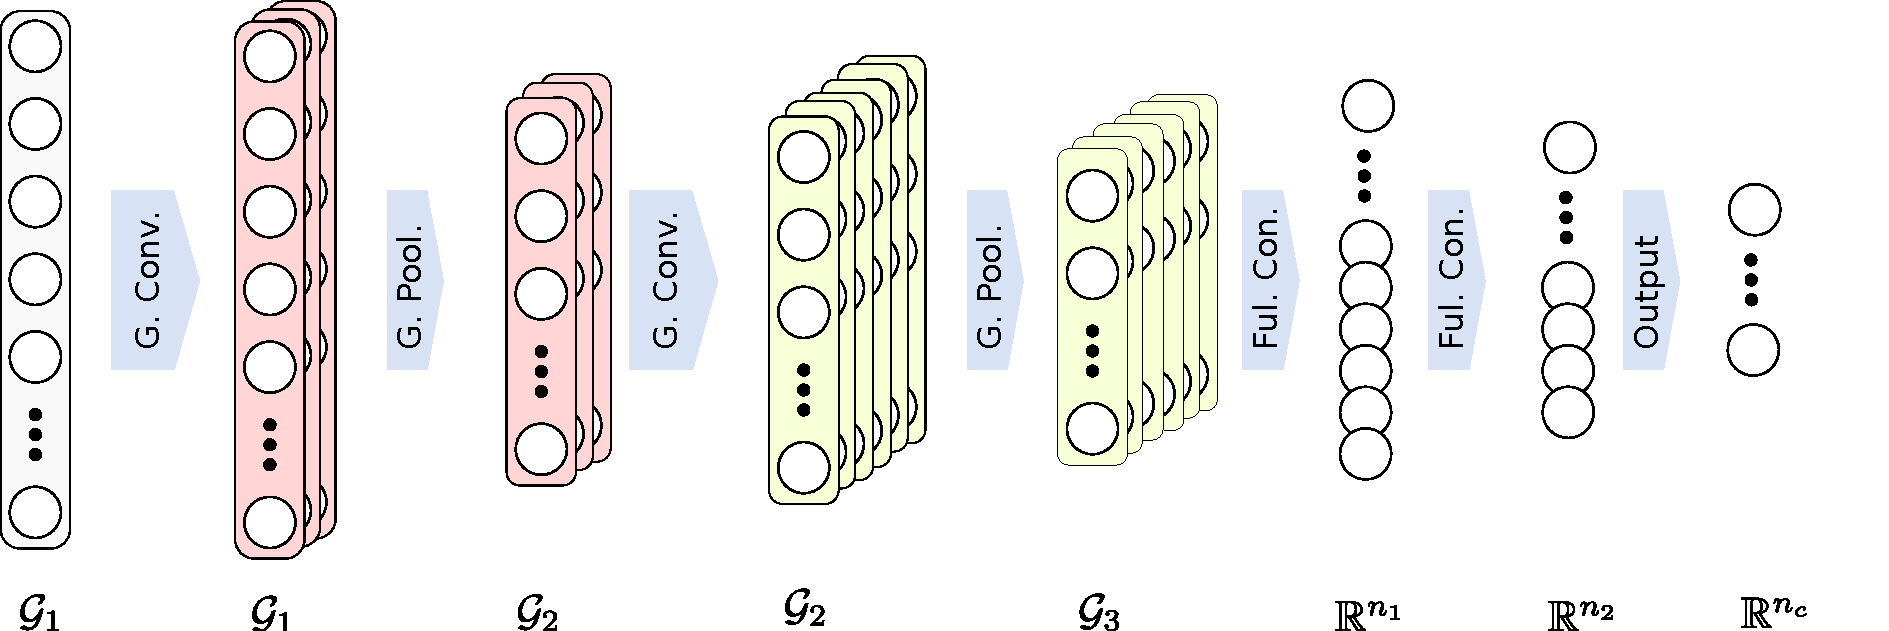
\includegraphics[width=\textwidth]{img/classifier.pdf}
    \caption{The architecture used to classify MNIST, with signal structure }
    \label{fig:mnist_classifier}
\end{figure}

We trained this architecture using a classic regularized cross entropy loss:
\begin{equation}
    \mathcal{L}(x,\hat{y},\theta) = -\sum_{i=1}^n \hat{y}\log P(y|x,\theta) + \alpha \sum_{j=1}^m \|\theta_j\|^2
\end{equation}
With a dataset of $n$ samples $\{(x_i, \hat{y_i})\}$, $m$ parameters $\theta_j$, and a regularization hyper-parameter $\alpha = 0.001$. We optimized this loss over the parameters using an AdaDelta optimizer \cite{Zeiler2012}, on mini-batch gradient descent (number of samples per batch = 300). On figure \ref{fig:training_curve}, we can see the training curve and the best test accuracy obtained of $\sim 96.9\%$. We stress out that in this work, the objective was to check that GCNN are able to learn from data, and not to perform a comparative study of the best GCNN architecture possible. Consequently, the performances of this classifier are not to be compared directly with other CNN performances, as no extensive tuning of architecture has been made to achieve the best possible accuracy. Moreover, it is worth noting that in the case of the classic LeNet5 architectures, each filter is of size $5\times5=25$, which is five times the length of the filters we used. To sum up, this test accuracy shows that the network has effectively learnt to classify the data set, and the tuning of the architecture could be subject to further work to obtain performances similar to the ones reached by classic architectures. 

\begin{figure}
    \centering
    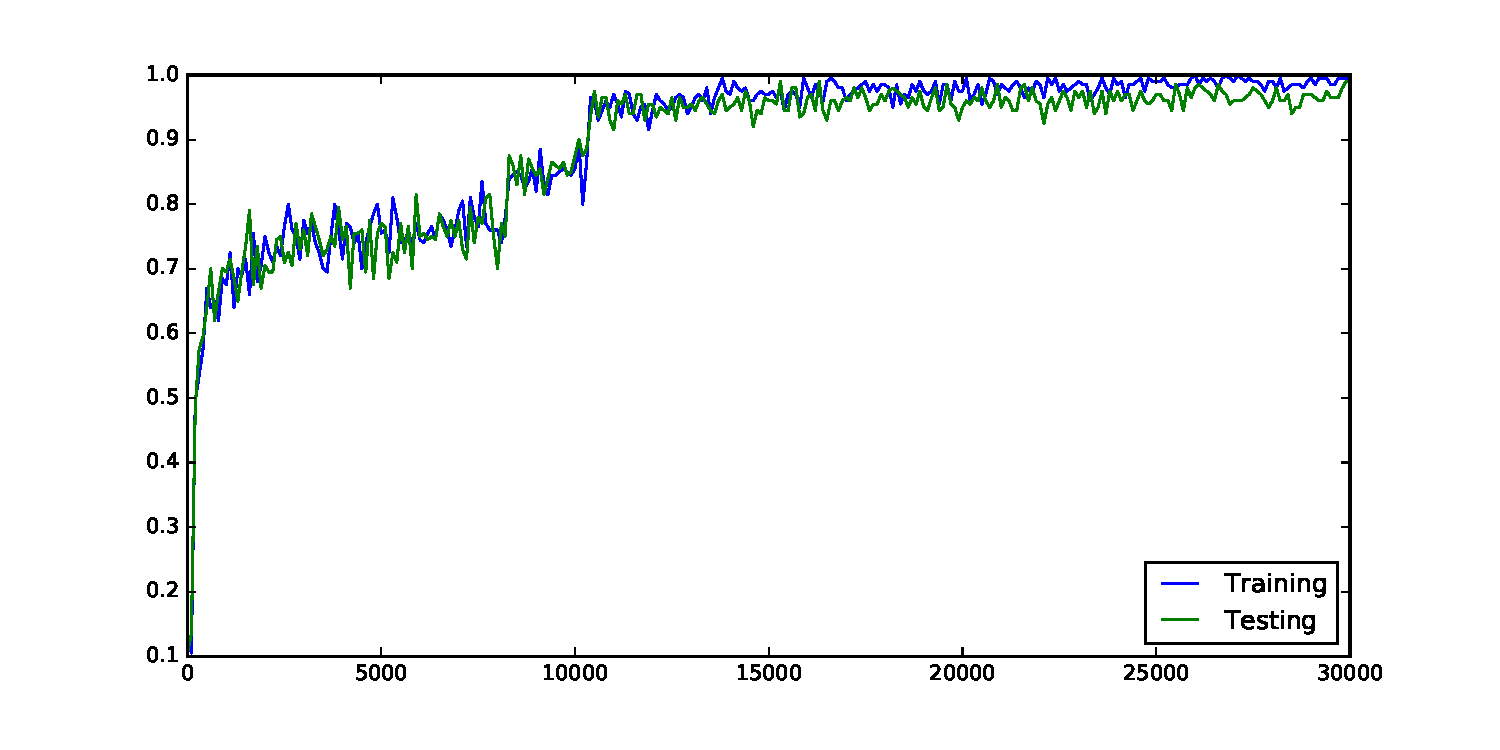
\includegraphics[width=\textwidth]{img/training_curve.pdf}
    \caption{Test and Train Accuracy through epochs. Final Test Accuracy: 96.9\%}
    \label{fig:training_curve}
\end{figure}

In a second time, once the principles of our implementation were validated by the first experiment, we have reimplemented our architecture using the two faster operations of Chebyshev Approximated Filters, and 1-D Max Pooling. Using this implementation allowed us to reach similar performance but in much shorter time as we can see on table \ref{tab:slow_fast}.

\begin{table}[]
    \centering
    \begin{tabular}{|l|c|}
        \hline
         Implementation & Epoch duration \\ \hline
         Graph Fourier Transform \& Transfert Matrix Pooling & 0.29s \\
         Chebyshev Approximation \& 1-D Max Pooling & 0.10s \\ \hline
    \end{tabular}
    \\
    \caption{Training epoch duration using slow and fast implementations, on GTX1080. The fast implementation allows a speedup of $\sim \times 3$.}
    \label{tab:slow_fast}
\end{table}


\subsection{Going Further with Autoencoding}

To push further the experiments already made in the paper, and to meet the final goal of this project, we have implemented a simple single filter autoencoder architecture, that we have trained in an unsupervised manner over the MNIST data. For the encoding part, we used the following Graph Convolutional stack:
\begin{itemize}
    \item Perform Graphical Filtering with largest Laplacian power $K_i=5$, and number of filters $n_i=1$
    \item Perform a ReLu Non-Linearity
    \item Perform a single Max Pooling to reduce the overall size about a factor $\sim 2$.
\end{itemize}
Concerning the decoder part, the data needs to be projected back to the larger graph at each stack. This is performed by simply projecting the signal values at coarsened nodes on their non-coarsened parents. This operation was easily implemented using the Transition matrix. Our Decoding Graph Convolutional stack was thus made of the following operations: 
\begin{itemize}
    \item Perform 2 Max UnPooling to enlarge the data of $\sim 2$
    \item Perform a ReLu Non-Linearity
    \item Perform a Graphical filtering with largest Laplacian power $K_i=5$, and number of filters $n_i=1$.
\end{itemize}

The overall architecture is composed of four Encoding Graph Convolutional stacks , and four Decoding Graph Convolutional stacks as depicted on figure \ref{fig:autoencoder}. We note that the embedded code is a vector of length $\sim60$ depending on the coarsening operation (compared to the input size $784$). 

\begin{figure}
    \centering 
    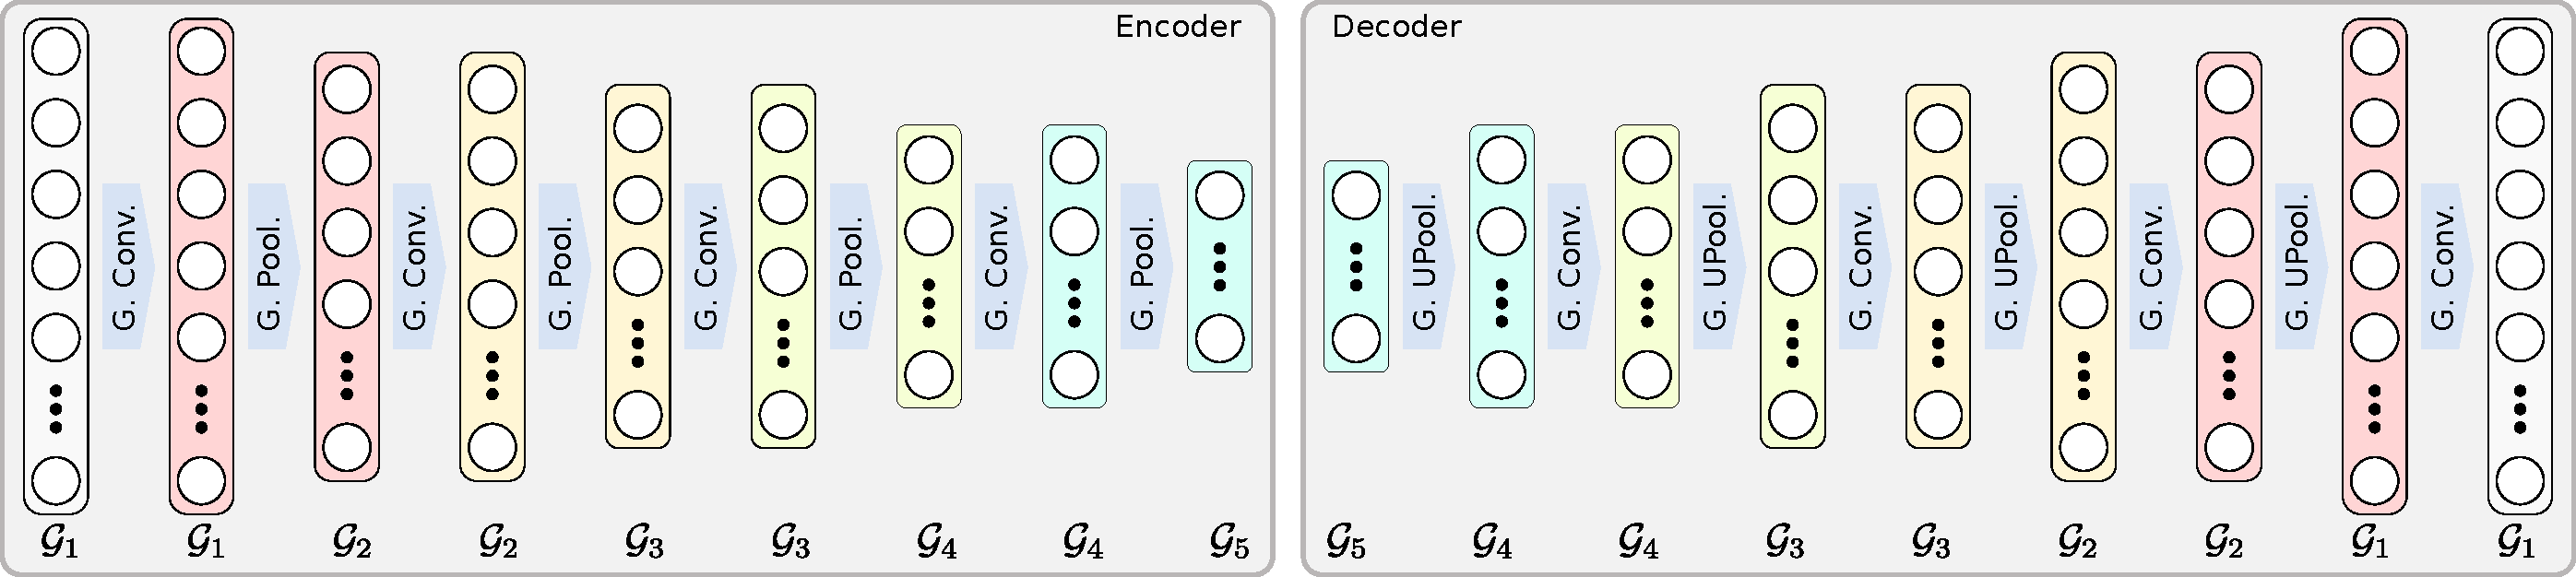
\includegraphics[width=\textwidth]{img/autoencoder.pdf}
    \caption{The architecture used to autoencode the MNIST DataSet, with signal structure.}
    \label{fig:autoencoder}
\end{figure}

We trained this architecture using a regularized L2-Distance:
\begin{equation}
    \mathcal{L}(x,\theta) = \|x-f(x)\|_2 + \alpha \sum_{j=1}^m \|\theta_j\|^2
\end{equation}
With $f(x)$, the output of the network for the training sample $x$. We trained the whole architecture from scratch, using again the AdaDelta Optimizer.

Using our trained autoencoder we were able to partially reconstruct samples as depicted on figure \ref{fig:reconstruction}. While keeping the overall shape of the digit, the reconstructions are still quite blurry, and our experiments have shown that the deeper the encoding, the blurrier the reconstruction was. To get deeper understanding of the learned embedded structure, we decoded some variable indicators of the embedded code (decode a $[0,0,1,0,0,\dots,0]$-like vector). When looking at the decoded plots of the first 16 indicators, we can see that the autoencoder has basically learnt to project the code signal from coarsened graph nodes to its parents nodes on the output space. In other words, it has learnt to approximate the identity operation. To our knowledge, it is a common pitfall in autoencoders, which can be overtaken using more complex forms of training (denoising for example). 

\begin{figure}
    \centering
    \subfigure[Reconstructed samples]{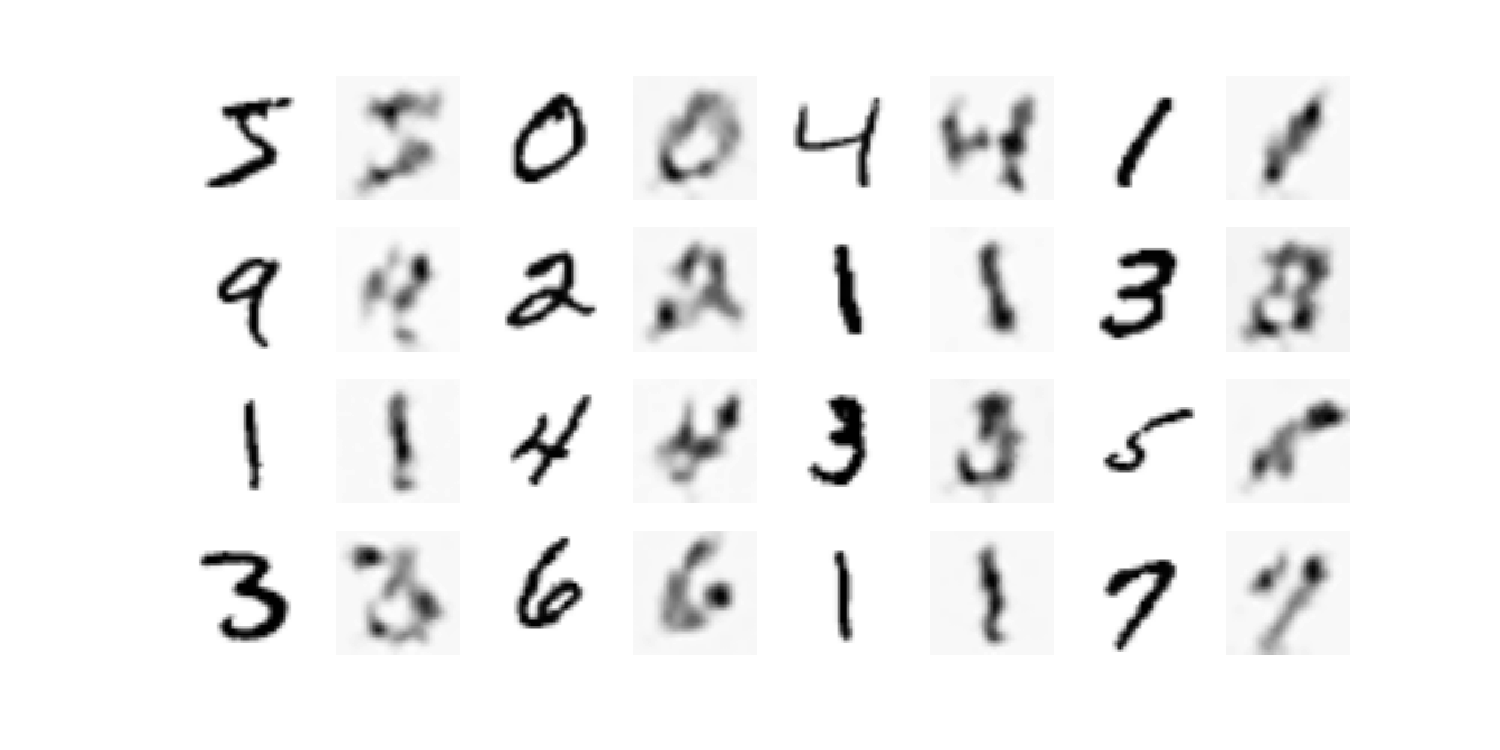
\includegraphics[width=0.66\textwidth]{img/reconstruction.pdf}}
    \subfigure[Code projection to output space]{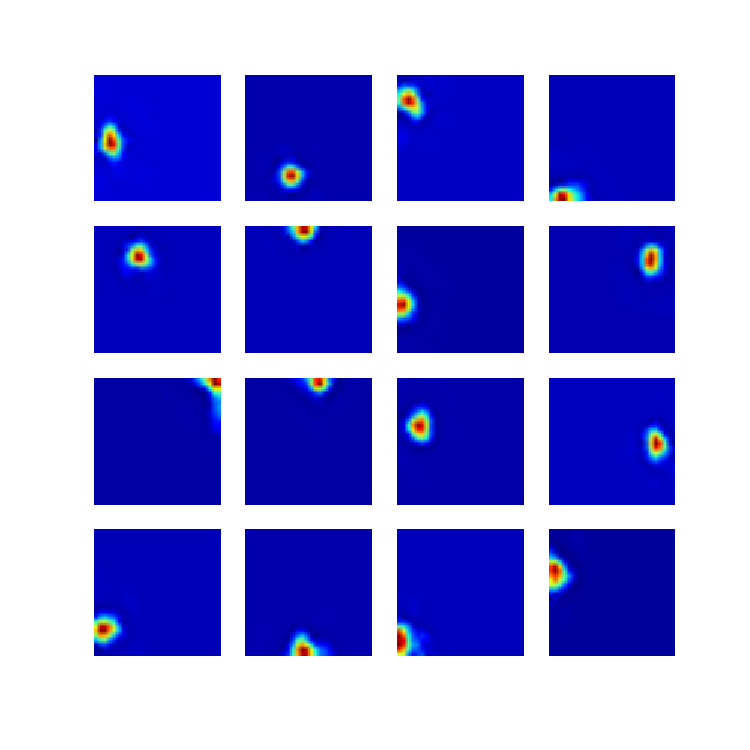
\includegraphics[width=0.33\textwidth]{img/code.pdf}}
    \caption{Reconstructed samples, and code variables projected to the output space}
    \label{fig:reconstruction}
\end{figure}

By the end of our experiments with autoencoders, it was still unclear if better behavior could be obtained using GCNN models. Once again, further work might be necessary to gain intuition about the potential of GCNN for autoencoding.

\section{Conclusion}
This project allowed us to work on the cutting edge topic of non-euclidean CNN. Interestingly, the ideas developed here can easily be extended to be used on data defined over Manifolds, as suggested in \cite{DBLP:journals/corr/BronsteinBLSV16}, which could lead to even larger applications. It is worth noting that since the beginning of this project, two unpublished (and not reviewed by us) papers have been proposed on the topic of GCNN and GCNN Autoencoders,  \cite{2016arXiv161107308K} \cite{DBLP:journals/corr/KipfW16}. The subject is hence in active research state, which explains why few experiments were made on the best architecture existing to tackle general Neural Networks problems. Hence the results produced during this project should be interpreted regarding the relative youth of those techniques, that do not benefit from a large research corpus as classic CNNs do. Nevertheless, regarding the results we had in our experiments, we are quite confident that great achievements will be made on this subject in a very near future. 

We would like to thank our adviser and reviewer \emph{Florian Strub}, for giving us the chance to work on such an interesting subject, and for his help to tackle the \texttt{tensorflow} implementation. The code we produced as part of this project is available at \url{https://github.com/ctiennot/graphConvNet}.



%\newpage

\bibliographystyle{abbrv}
\bibliography{biblio}

\end{document}

